%! Author = paulsen
%! Date = 10.09.23

\begin{frame}{Einführung}
    \section{Einführung}\label{sec:einfuhrung}
\end{frame}

\begin{frame}{Vorstellung}
    \subsection{Vorstellung}\label{subsec:vorstellung}

    \underline{\textbf{Paul Seidel}}

    \begin{itemize}
        \item Internet Computing
        \item Linux seit 3 Jahren in der Uni \& Privat
        \item Ja, ich benutze auch Windows :)
    \end{itemize}

    \pause
    \vspace{0.5cm}
    \begin{alertblock}{Diskussion}
        Was ist euer Hintergrund?
    \end{alertblock}

\end{frame}
\begin{frame}{Erwartungen}
    \subsection{Erwartungen}\label{subsec:erwartungen}
    Eventuell Vorurteile?
    \vspace{0.5cm}\pause
    \newline
    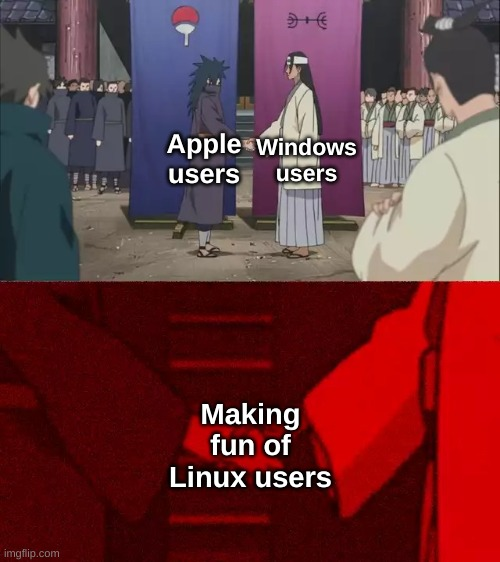
\includegraphics[width=6cm]{Meme_Making-Fun-Of-Linux}
\end{frame}

\begin{frame}{Erwartungen}
    \begin{itemize}
        \item \begin{quote}
                  Linux ist was für Nerds!
        \end{quote}\pause
        \item \begin{quote}
                  Da macht man alles in der "Hacker"-Konsole!
        \end{quote}\pause
        \item \begin{quote}
                  Das ist mir zu viel Neuland!
        \end{quote}
    \end{itemize}

    \pause
    \vspace{0.5cm}
    \begin{alertblock}{Diskussion}
        Wie sieht es bei euch aus?
    \end{alertblock}

\end{frame}

\begin{frame}{Ziele}
    \subsection{Ziele}\label{subsec:ziele}

    \begin{enumerate}
        \item Schnelle Installation\pause
        \item Nutzung von Software\pause
        \item Umgang mit der Konsole\pause
        \item Systemkonfiguration\pause
        \item Beheben von Problemen\pause
        \item Gute Kenntnisse zum eigenständigen Arbeiten\pause
    \end{enumerate}

\end{frame}